\chapter{Predikce}

\section{Úvod}

Předpokládejme, že máme k dispozici časovou řadu $x_1, x_2, ..., x_N$. Cílem predikce je odhadnout budoucí hodnoty $x_{N + k}$. Parametr $k > 0$ je nazýván časem predikce (lead time). Odhad $x_{N + k}$ učiněný v čase $N$ pro $k$ časových kroků dopředu budeme v následujícím textu označovat jako $\hat{x}(N, k)$.

Je třeba si uvědomit, že predikce časových řad není dána direktivním postupem, na jehož konci stojí jeden jediný správný výsledek. Analytik by měl být připraven získané odhady v případě potřeby modifikovat tak, aby co nejlépe odrážely informace, které má k dispozici. Je také vhodné nespoléhat pouze na jeden model a jednu sadu předpokladů. Naopak, je žádoucí s pomocí různých modelů či na základě různých předpokladů získat několik odhadů. Jejich vzájemným porovnáním si pak analytik může učinit představu o jejich spolehlivosti.

Predikce nemusí být vždy založené na kvantitativních metodách, ale mohou také odrážet expertní názor jednotlivce nebo skupiny jednotlivců.\footnote{Speciální expertní metodou predikce je tzv. technika Delfské věštírny, kdy se v několika kolech snaží skupina expertů dosáhnout konsenzu formou řízené diskuze.} Nicméně statistici dávají většinou přednost kvantitativním metodám. V praxi dochází často ke kombinaci obou přístupů, kdy jsou výstupy kvantitativních metod konfrontovány s názory expertů na danou problematiku.

Kvantitativní prediktivní metody mohou být jedno či vícerozměrné. V případě jednorozměrných prediktivních metod je odhad dané veličiny založen pouze na jejích předchozích pozorováních. Jinými slovy $\hat{x}_{N, k}$ je pouze funkcí $x_N, x_{N-1}, ...$. Proto někdy jednorozměrné prediktivní metody nazýváme také naivními metodami popř. metodami projekce. Naproti tomu v případě vícerozměrných prediktivních metod je odhad zkoumané veličiny funkcí jedné nebo několika jiných časových řad, které nazýváme prediktory.\footnote{V ekonometrii se také často používá pojem nezávislé popř. vysvětlující veličiny.}

Kvantitativní prediktivní metody mohou být také členěny na automatické a manuální, podle toho, zda vyžadují vstup ze strany analytika či nikoliv. Automatické metody jsou vhodné při velkém množství zpracovávaných časových řad popř. při nedostatečné odbornosti analytika. Naproti tomu manuální metody vyžadují značnou míru zkušenosti pro jejich aplikaci. Tyto metody se tak nehodí pro masové zpracování dat, nicméně v řadě případů přinášejí lepší výsledky než automatické metody.

\section{Jednorozměrné prediktivní metody}

\subsection{Extrapolace trendové křivky}

U dlouhodobých predikcí je často užitečné nakalibrovat trendovou křivku na pozorovanou časovou řadu a následně extrapolovat. Jako trendovou křivku lze použít polynomickou, exponenciální, logistickou či Gompertzovu křivku. Pro smysluplnou kalibraci trendu je však vyžadováno alespoň sedmi až desetileté období. Dále platí pravidlo, že časový horizont predikce by neměl přesahovat polovinu délky historického okna, které jsme použili pro kalibraci trendové křivky.

Nevýhodou této metody je skutečnost, že s výjimkou míry shody (goodness-of-fit), neexistuje žádný logický důvod, proč bychom při kalibraci trendu měli preferovat konkrétní křivku. V praxi se tak často dostáváme do situace, kdy jsou z pohledu míry shody dvě křivky téměř rovnocenné, nicméně jimi implikované predikce se značně liší.

\subsection{Exponenciální vyhlazení}

Exponenciální vyhlazení (exponencial smoothing) by mělo být aplikováno ve své základní podobě pouze na časové řady, které nevykazují trend ani sezónnost. Nicméně jak trend tak sezónnost lze z časové řady odstranit a získat tak stacionární časovou řadu.

V případě stacionární časové řady $x_1, x_2, ..., x_N$ je přirozené odhadnout $x_{N+1}$ jako vážený průměr minulých pozorování, tj. jako
\begin{equation}
\hat{x}(N, 1) = c_0 x_N + c_1 x_{N-1} + c_2 x_{N-2} + ...,
\end{equation}
kde $\{c_i\}$ jsou váhy. Intuitivně by váha měla být tím větší, čím aktuálnější jsou pozorování. Jedním z řešení je tak aplikovat tzv. geometrické váhy, kde
\begin{equation}
c_i = \alpha(1 - \alpha)^i \quad i = 0, 1, ...
\end{equation}
a $0 < \alpha < 1$ je konstanta. Rovnice (5.1) tak získá podobu
\begin{equation}
\hat{x}(N, 1) = \alpha x_N + \alpha(1 - \alpha)x_{N-1} + \alpha(1 - \alpha)^2 x_{N - 2} + ...~.
\end{equation}
Rovnice (5.3) se dá rekurzivně zapsat jako
\begin{multline}
\hat{x}(N, 1) =\\
\alpha x_N + (1 - \alpha)[\alpha x_{N - 1} + \alpha x_{N - 1} + \alpha(1 - \alpha)^2 x_{N-2} + ...~]\\
=\alpha x_N + (1 - \alpha) \hat{x}(N - 1, 1).
\end{multline}
Proces popsaný rovnicí (5.4) pak nazýváme exponenciálním vyhlazením. Pojem ``exponenciální'' vychází ze skutečnosti, že jednotlivé váhy klesají exponenciálně v čase.

Rovnice (5.4) je někdy také prezentována v tzv. ``korekčním'' tvaru (error-correction form)
\begin{equation}
\hat{x}(N, 1) = \alpha[x_N - \hat{x}(N - 1, 1)] + \hat{x}(N - 1, 1) = \alpha e_N  + \hat{x}(N - 1, 1),
\end{equation}
kde $e_N = x_N - \hat{x}(N - 1, 1)$ je chyba predikce v čase $N$.

Lze dokázat, že model exponenciální vyhlazení je optimální, pokud má podkladová časová řada podobu
\begin{equation}
X_t = \mu + \alpha \sum_{j < r}Z_j + Z_t.
\end{equation}
Tato časová řada je nestacionární, nicméně pomocí diference prvního řádu získáme proces klouzavého průměru prvního řádu. Jinými slovy, $X_t$ je ARIMA(0, 1, 1) procesem.

Hodnota parametru $\alpha$ závisí na vlastnostech podkladové časové řady. Hodnoty v rozmezí 0.1 až 0.3 znamenají, že predikce je závislá na poměrně velkém počtu minulých pozorování. Naproti tomu hodnotu blízké jedné znamenají, že pro účely predikce jsou relevantní pouze nejaktuálnější pozorování.

Hodnotu parametru $\alpha$ lze odhadnout podobně jako v případě odhadů parametru MA procesu. Součet čtverců chyby predikce je vypočten pro různé hodnoty $\alpha$ a následně je vybrána taková hodnota parametru, která tento součet minimalizuje. Pro danou hodnotu $\alpha$ tedy nejprve vypočteme
\begin{equation}
\begin{aligned}
\hat{x}(1, 1) = x_1\\
e_2 = x_2 - \hat{x}(1, 1)\\
\hat{x}(2, 1) = \alpha e_2 + \hat{x}(1, 1)\\
e_3 = x_3 - \hat{x}(2, 1)\\
...\\
e_N = x_N - \hat{x}(N - 1, 1)
\end{aligned}
\end{equation}
a následně pak určíme součet čtverců reziduí $\sum_{i = 2}^N e^2_i$. Tento postup aplikujeme na všechny hodnoty $\alpha$ v intervalu 0 až 1 s krokem např. 0.1 a vybereme takovou hodnotu $\alpha$, která minimalizuje $\sum_{i = 2}^N e^2_i$. Obvykle je křivka součtu čtverců reziduí v okolí minima relativně plochá a výběr přesné hodnoty $\alpha$ tak není kritický.

\subsection{Holt-Wintersova metoda}

Holt-Wintersova metoda je zobecněním metody exponenciálního vyhlazení aplikované na časové řady obsahující trend a sezónnost. Jedná se o metodu, která je přímočará a v praxi často používaná.

Předpokládejme měsíční pozorování. Nechť $L_t, T_t$ a $I_t$ představují index úrovně, trendu a sezónnosti v čase $t$. Dále nechť $\alpha, \gamma$ a $\delta$ označují tři parametry vyhlazení, které typicky volíme z intervalu $(0, 1)$. Jestliže je sezónnost multiplikativního charakteru a máme k dispozici pozorování $x_t$, pak lze $L_t, T_t$ a $I_t$ zaktualizovat pomocí následujících rovnic
\begin{equation}
\begin{aligned}
L_t = \alpha(x_t / I_{t - 12}) + (1 - \alpha)(L_{t-1} + T_{t - 1})\\
T_t = \gamma(L_t - L_{t - 1}) + (1 - \gamma) T_{t - 1}\\
I_t = \delta(x_t / L_t) + (1 - \delta) I_{t - 12}
\end{aligned}
\end{equation}
a predikce v čase $t$ má podobu
\begin{equation}
\hat{x}(t, k) = (L_t + k T_t) I_{I - 12 + k}
\end{equation}
pro $k = 1, 2, ..., 12$. Pro případ aditivní sezónnosti existují analogické vzorce.

Před aplikací Holt-Wintersovy metody bychom měli analyzovat graf časové řady s cílem určit, zda-li má případná sezónnost aditivní nebo multiplikativní charakter. Pokud sezónní frekvence nepokrývá 12 období, ale např. pouze 4 období, je třeba výše uvedené vzorce upravit.

Holt-Wintersovu metodu lze implementovat v následujících čtyřech krocích.
\begin{itemize}
\item Nejprve stanovíme počáteční hodnoty pro $L_t, T_t$ a $I_t$ na začátku časové řady, tj. pro $t = 0$.
\item Pomocí minimalizace $\sum e_t^2$ odhadneme hodnoty parametrů $\alpha, \gamma$ a $\delta$.
\item Rozhodneme, zda-li normalizovat sezónní indexy, viz. kapitola 2.6.
\item Zvolíme automatickou popř. manuální verzi metody.
\end{itemize}

\subsection{Box-Jenkinsova metoda}

AR, MA a ARMA modely existovaly dlouho před ARIMA modelem. Hlavním přípěvkem Boxe a Jenkinsona byla formulace obecného postupu pro predikci časových řad a důkaz, že pomocí diference lze rozšířit použití ARMA modelu také na nestacionární časové řady. Tak se ``zrodil'' ARIMA model, který je základem tzv. Box-Jenkinsovy metody.

Prvním krokem Box-Jenkinsovy metody je ``konverze'' nestacionární časové řady na stacionární pomocí diference. Posouzení stacionarity se většinou opírá o analýzu korelogramů diferencovaných časových řad. Jako optimální diferenci označujeme takovou, která (a) z časové řady dostatečným způsobem odstraňuje sezónnost a (b) po jejíž aplikaci klesá korelogram podkladové řady dostatečně rychle k nule. V případě nestacionárních časových řad zatížených pouze trendem zpravidla postačuje diference prvního řádu. V případě časové řady, která navíc obsahuje sezónnost s měsíční aditivní periodou, je třeba použít diferenci $\nabla \nabla_{12}$; v případě sezónnosti s měsíční multiplikativní periodou pak diferenci $\nabla_{12}^2$. Výslednou časovou řadu v následujícím textu označujeme jako $\{w_t; t = 1, ..., N - c\}$, kde $c$ představuje počet pozorování ztracených v důsledku diference. Např. pro $\nabla \nabla_{12}$ je $c$ rovno 13.

Pokud data nevykazují sezónnost, můžeme na ně nakalibrovat ARMA model. Postup kalibrace byl načrtnut v předchozí kapitole. Pokud data sezónnost vykazují, lze na nich nakalibrovat SARIMA model. ``Rozumné'' hodnoty $p, P, q$ a $Q$ jsou odhadnuty na základě korelogramu a parciální autokorelační funkce časové řady $\{w_i\}$, která je z původní časové řady odvozena pomocí diference. Hodnoty $p$ a $q$ jsou vybrány s ohledem na několik prvních hodnot $r_k$ tak, jak bylo popsáno v kapitole 4. Hodnoty $P$ a $Q$ jsou zvoleny na základě analýzy $r_k$ pro $k = 12, 24, ...$.\footnote{Předpokládáme sezónní periodicitu 12 časových období.} Pokud je např. $r_{12}$ ``vysoké'' a $r_{24}$ naopak ``nízké'', zvolíme $P = 0$ a $Q = 1$, protože tento SARIMA model má podobnou autokorelační funkci.

Pokud jsme ``intuitivně'' vybrali vhodnou formu SARIMA modelu, můžeme jeho parametry odhadnout pomocí metody nejmenšího součtu čtverců reziduí podobně jako v případě ARMA modelu. V případě sezónních časových řad je vhodné odhadnout počáteční hodnoty $a_t$ a $w_t$ pomocí zpětné predikce (backforcasting), spíše než je položit rovné nule. Pokud model obsahuje parametr sezónního klouzavého průměru blízký jedné, může být zapotřebí několika cyklů dopředné a zpětné iterace.

Ať už data vykazují sezónnost či nikoliv, je žádoucí zkontrolovat vhodnost zvoleného modelu pomocí testování náhodnosti reziduí. Z korelogramu reziduí je možné odvodit, zda-li jsou některé koeficienty významně odlišné od nuly a zda-li je tak třeba ARIMA model odpovídajícím způsobem modifikovat.

V okamžiku, kdy máme vybrán a nakalibrován vhodný ARIMA model, můžeme přistoupit k predikci. Predikce $X_{N + k}$ v čase $N$ má charakter podmíněné střední hodnoty $\hat{x}(N, k) = E(X_{N + k}| X_N, X_{N - 1}, ...)$. Při kvantifikaci $\hat{x}(N, k)$ pak využíváme skutečnosti, že ``nejlepší'' predikce všech budoucích $Z$ je nula, tj. $E(Z_{N + k}|X_N, X_{N - 1}, ...) = 0$ pro všechna $k$.

Box a Jenkins (1970) popisují následující tři metody predikce. Tyto metody předpokládají znalost rovnice modelu.
\bigbreak
\noindent
\textbf{(a) Iterační metoda}

Pokud známe rovnici modelu, lze $\hat{x}(N,k)$ získat nahrazením (1) budoucích hodnot $Z$ nulou, (2) budoucích hodnot $X$ jejich podmíněnou střední hodnotou a (3) minulá $X$ a $Z$ jejich skutečně pozorovanými hodnotami.

Jako příklad uvažujme model SARIMA(1, 0, 0)(0, 1, 1)$_{12}$
\begin{equation}
X_t = X_{t - 12} + \alpha(X_{t - 1} - X_{t - 13}) + Z_t + \theta Z_{t - 12}.
\end{equation}
První dvě predikce $X$ lze vypočíst jako
\begin{equation}
\hat{x}(N, 1 ) = x_{N - 11} + \alpha (x_N - x_{N - 12}) + \theta z_{N - 11},
\end{equation}
\begin{equation}
\hat{x}(N, 2) = x_{N - 10} + \alpha[\hat{x}(N, 1) - x_{N - 11}] + \theta z_{N - 10}.
\end{equation}
Následující predikce lze vypočíst analogickým způsobem.
\bigbreak
\noindent
\textbf{(b) Metoda založená váhách $\psi$}

Pro výpočet predikce lze také použít váhy $\psi$ definované v rovnici (3.70), které jsou obzvláště vhodné pro výpočet rozptylu predikované hodnoty. Protože
\begin{equation}
X_{N + k} = Z_{N + k} + \psi_1 Z_{N + k - 1} + ...,
\end{equation}
je zřejmé, že $\hat{x}(N, k)$ je rovno $\sum_{j = 0}^{\infty} \psi_{k + j} Z_{N - j}$ (tj. do rovnice nezahrnujeme budoucí $Z$). Dále je z této rovnice zřejmé, že rozptyl $\hat{x}(N, k)$ je roven $Z_{N + k} + \psi_1 Z_{N + k - 1} + ... + \psi_{k - 1} Z_{N + 1} = (1 + \psi_1^2 + ... + \psi_{k - 1}^2) \sigma_Z^2$.
\bigbreak
\noindent
\textbf{(c) Metoda založená váhách $\pi$}

Kromě vah $\psi$ lze také použít váhy $\pi$ definované rovnicí (3.72). Protože
\begin{equation}
X_{N + k} = \pi_1 X_{N + k - 1} + ... + \pi_k X_N + ... + Z_{N + k},
\end{equation}
je zjevné, že
\begin{equation}
\hat{x}(N, k) = \pi_1 \hat{x}(N, k - 1) + \pi_2 \hat{x}(N, k - 2) + \pi_k + X_N + \pi_k X_{N - 1} + ...
\end{equation}
Hodnoty $\hat{x}(N, k)$ lze vypočíst rekurzivně tak, že budoucí hodnoty $X$ budeme postupně nahrazovat jejich predikcemi. Jinými slovy, abychom mohli vypočíst $\hat{x}(N, k)$, musíme mít k dispozici všechny předchozí predikce $\hat{x}(N, k - 1), \hat{x}(N, k - 2), ..., \hat{x}(N, 1)$.
\bigbreak

V praxi však bohužel modelovou rovnici neznáme, a proto je třeba nejprve její parametry (popř. také váhy $\psi$ a $\pi$) odhadnout. Následně je také třeba odhadnout minulé hodnoty $Z$ pomocí reziduí daného modelu. Např. pro výše uvažovaný model SARIMA(1, 0, 0)(0, 1, 1)$_{12}$ tak získáváme
\begin{equation}
\hat{x}(N, 1) = x_{N - 11} + \hat{\alpha} (x_N - x_{N - 12}) + \hat{\theta} \hat{z}_{N - 11}.
\end{equation}

Často dochází k situaci, kdy dva rozdílné ARIMA modely jsou schopny podobným způsobem replikovat pozorovaná data, nicméně predikce na nich založené se významně liší. Vybrat ``správný'' model pak může být poměrně obtížné. Další komplikací je skutečnost, že výše uvedené postupy vyžadují několik let dlouhou historickou řadu (alespoň 50 pozorování v případě měsíční dat, pokud tato data vykazují sezónnost).

\subsection{Postupná autoregrese}

Na metodu postupné autoregrese (stepwise autoregression) navrženou Grangerem a Newboldem (1980) lze nahlížet jako na ``podmnožinu'' Box-Jenkinsovy metody, která má však tu výhodu, že ji lze zcela automatizovat. Tato metoda je založená na skutečnosti, že AR modely lze v porovnání s MA a ARMA modely mnohem snáze nakalibrovat.\footnote{I když AR model může vyžadovat větší počet parametrů, aby byl schopen obdobným způsobem replikovat historická data.}

Postup Granger-Newboldovy metody je následující. Nejprve je pomocí diference odstraněn případný lineární trend. Pak je zvoleno maximální zpoždění $p$. Granger a Newbold navrhují zvolit $p = 13$ pro čtvrtletní a $p = 25$ pro měsíční data. Následně je určen nejlepší autoregresní model založený pouze na jedné zpožděné veličině, tj.
\begin{equation}
W_t = \mu + \alpha_k^{(1)} W_{t - k} + e_t^{(1)} \quad 1 \le k \le p,
\end{equation}
kde $W_t = X_t - X_{t - 1}$. V dalších krocích je nalezen nejlepší autoregresní model pro 2, 3, ... zpožděné veličiny. S tím, jak postupně přidáváme další zpožděné veličiny, klesá součet čtverců reziduí. Procedura je ukončena, pokud redukce součtu čtverců reziduí klesne pod určitou zvolenou hranici. Příslušný model je prohlášen za ``optimální''.

\section{Vícerozměrné prediktivní metody}

\subsection{Vícerozměrná lineární regrese}

Ve vícerozměrném lineárním regresním modelu je závislá veličina vyjádřena jako lineární kombinace vícero nezávislých veličin. Do modelu je možné zahrnout nejen současné ale také zpožděné nezávislé veličiny. Zahrnutí zpožděných závislých veličin v roli nezávislých veličin je také možné, i když tím měníme charakter modelu.

Vysoký výpočetní výkon a dostupnost ekonometrických balíčků má za následek, že je do regresního modelu zahrnováno stále více nezávislých veličin, což vede k tzv. ``přeučení'' (overfitting) modelu. Přeučení modelu se projevuje tím, že ačkoliv je model schopen velmi dobře replikovat pozorovaná data (projevuje se vysokou mírou shody reprezentovanou např. $R^2$), jeho prediktivní schopnosti jsou velmi špatné. Optimální počet nezávislých veličin se odvíjí od délky historické časové řady, na které model kalibrujeme, a od charakteru problému, který se jím snažíme popsat. Obecně však platí, že pokud ve vícerozměrném regresním modelu použijeme více než šest až sedm nezávislých veličin, měli bychom k tomu mít dobrý důvod.

Dalším problémem, který souvisí s velkým počtem nezávislých proměnných, je skutečnost, že tyto veličiny jsou v praxi často vzájemně korelované, což má za následek velkou směrodatnou chybu odhadnutých parametrů regresního modelu. Jinými slovy, hodnoty odhadů těchto parametrů se mohou významných způsobem změnit i při relativně malé změně modelu či dat, na kterých je model kalibrován.

Někdy mohou být důležité nezávislé veličiny v rámci historického okna, na kterém kalibrujeme regresní model, relativně neměnné. Vliv těchto veličin v rámci odhadnutého modelu je pak poměrně zanedbatelný a jejich ``adekvátní'' zohlednění přinejmenším problematické. Jako příklad uveďme situaci, kdy společnost uvažuje o radikálním navýšení svých marketingových výdajů, a ráda by tak zkonstruovala regresní model, který by popisoval očekávaný vývoj tržeb v závislosti na těchto výdajích. Nicméně jestliže byly marketingové výdaje firmy v minulosti konstantní, není možné odhadnout vliv těchto výdajů na vývoj tržeb.

Pravděpodobně nejdůležitějším problémem vícenásobného regresního modelu je tzv. autokorelace chybového členu. Teorie odhadu regresního modelu předpokládá, že chybový člen (a tím pádem také rezidua, která jsou jeho odhadem) má charakteristiku tzv. bílého šumu (white noise). V praxi však tento předpoklad často není splněn. Autokorelaci lze pak (alespoň částečně) z modelu odstranit zahrnutím zpožděných veličin. Podrobnější rozbor této problematiky však přesahuje záběr naší knihy.

\subsection{Ekonometrické modely}

Ekonometrický model předpokládá, že ekonomický systém může být popsán nikoliv jednou rovnicí ale soustavou tzv. simultánních rovnic. Ekonomové pak rozlišují mezi tzv. exogenními veličinami, které ovlivňují systém a přitom nejsou systémem sami ovlivňovány, a tzv. endogenní veličiny, které mezi sebou vzájemně interagují. Soustava simultánních rovnic zahrnující $k$ závislých (endogenních) veličin $\{Y_i\}$ a $g$ předurčených (exogenních) veličin $\{X_i\}$ může být vyjádřena jako
\begin{equation}
Y_i = f_i(Y_1, ..., Y_{i - 1}, Y_{i + 1}, ..., Y_{k}, X_1, ..., X_g) + e \quad i = 1, 2, ..., k.
\end{equation}
Některé z exogenních veličin mohou být zpožděné veličiny $Y_i$.

Řešením výše uvedené soustavy simultánních rovnic získáme tzv. redukovaný systém rovnic ve tvaru
\begin{equation}
Y_i = F_i(X_1, ..., X_g) + e \quad i = 1, 2, ..., k.
\end{equation}

Detailnější popis principů řešení soustavy simultánních rovnic a problémů s tím spojených přesahují záběr této knihy.

\section{Porovnání prediktivních metod}

\subsection{Hromadné porovnání prediktivních metod}

V minulosti bylo provedeno několik studií, které se zabývaly porovnáním jednorozměrných prediktivních metod s ohledem na přesnost jejich predikce. Vzhledem k rozdílnosti přístupů a dat, na kterých bylo srovnání uskutečněno, není překvapující, že se závěry jednotlivých studií často rozchází. Některé studie došly k závěru, že nejlepší obecnou prediktivní metodou je Box-Jenkinsova metoda, jiné studie preferovali jiné jednorozměrné prediktivní metody.

Přesnost predikce je však pouze jedním z aspektů, proč bychom měli preferovat určitou prediktivní metodu. Dalšími aspekty jsou složitost její implementace a interpretace. Zejména v situaci, kdy jsme nuceni pracovat s velkým počtem časových řad, je žádoucí, aby prediktivní metoda mohla být kalibrována automaticky. V tomto případě se jako nejhodnější z jednorozměrných prediktivních metod zdá být Holt-Wintersova metoda, která je navíc relativně spolehlivá a snadno pochopitelná.

\subsection{Volba vhodné manuální metody}

V případě složitějších modelů může být lidský faktor rozhodující pro kvalitu predikce. V případě jednorozměrných prediktivních metod však obvykle není rozdíl mezi automatickou a ``manuální'' kalibrací modelu zásadní, což zvýhodňuje Holt-Wintersovu metodu před Box-Jenkinsovou metodou. Obecně platí, že použití Box-Jenkonsovy metody může být přínosem, pokud (1) má analytik dostatečné zkušenosti, (2) cíl analýzy ospravedlňuje použití složitější metody a (c) variace časové řady není primárně dána trendem nebo sezónností.

\subsection{Strategie pro aplikaci jednorozměrné manuální prediktivní metody}

\begin{enumerate}
\item Získejte informace o charakteru a vlastnostech podkladové časové řady. Definujte si jednoznačně cíle analýzy.
\item Graficky si znázorněte časovou řadu a zaměřte svou pozornost na trend, sezónnost, odlehlá pozorování, nespojitosti a změny ve střední hodnotě nebo rozptylu.
\item V případě potřeby očistěte časovou řadu o odlehlá pozorování. Zvažte možnost transformace dat např. aplikací přirozeného logaritmu.
\item Rozhodněte, zda-li sezónnost v časové řadě (a) není přítomna, (b) má multiplikativní či (c) aditivní charakter.
\item Rozhodněte, zda-li trend v časové řadě (a) není přítomen, (b) je globálně lineární, (c) je lokálně lineární nebo (d) je nelineární.
\item Na časovou řadu nakalibrujte vhodný model.
\begin{itemize}
\item Pokud je časová řada nespojitá, jako např. v případě obrázku (5.1a), není vhodné aplikovat jednorozměrnou prediktivní metodu.
\item Pokud časová řada zahrnuje sezónnost, jako např. v případě obrázku (5.3), je vhodná Holt-Wintersova metoda. Je třeba odhadnout správnou formu sezónnosti a parametry vyhlazení je možné odhadnout skrze optimalizaci předpovědí na následující časový krok.
\item Pokud časová řada obsahuje krátkodobou korelaci, jako je tomu např. v případě obrázku (5.1b), je třeba porozumět charakteru autokorelace. Pro tento typ časových řad lze doporučit Box-Jenkinsovu metodu.
\item Pokud časová řada vykazuje exponenciální růst, jako je tomu např. v případě obrázku (5.1c), je možné exponenciální trend odstranit popř. na ni nakalibrovat model, který v sobě zahrnuje exponenciální či kvadratický trend. Je však třeba zvýšené opatrnosti, protože exponenciální trend nemůže ve většině případů pokračovat do nekonečna. Proto je vhodné kalibrovaný model zkonzultovat s odborníky.
\end{itemize}
\item Zkontrolujte adekvátnost nakalibrovaného modelu a v případě potřeby jej modifikujte.
\item Využijte zkalibrovaný model k výpočtu predikcí.
\end{enumerate}

\begin{figure}[htp]
\centering
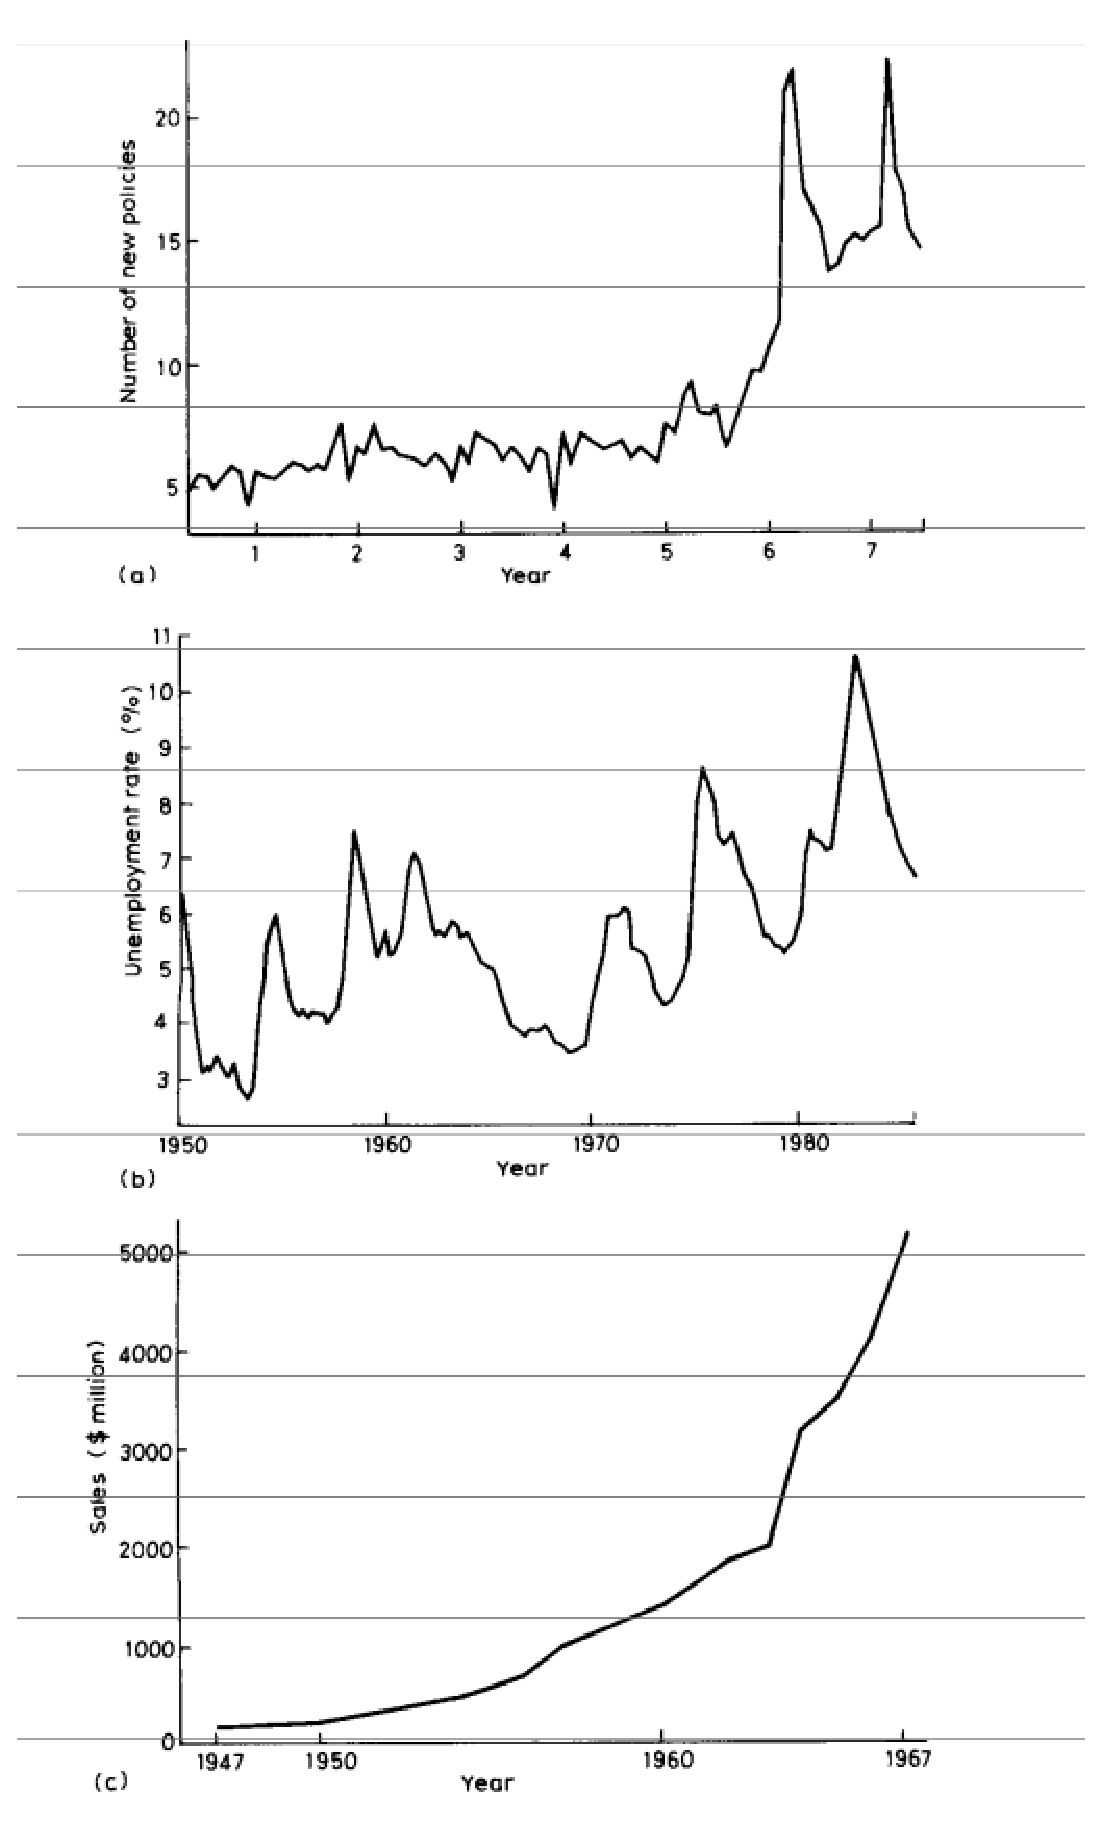
\includegraphics[scale = 0.55]{pictures/figure_5_1.eps}
\caption{Příklady časových řad. (a) Nespojitost - počet nově uzavřených pojistných smluv (v tisících za měsíc) v rámci jedné pobočky; (b) Krátkodobá autokorelace - míra nezaměstnanosti v USA; (c) Exponenciální trend - celosvětový vývoj ročních tržeb společnosti IBM}
\label{figure_5_1}
\end{figure}

\subsection{Shrnutí}

\begin{enumerate}
\item Model, který nejlépe replikuje historická data, nemusí oproti ostatním modelům vykazovat nižší chybu predikce. V praxi často platí, že složité modely, které jsou schopné velmi dobře replikovat historická data, nejsou z hlediska predikce lepší než výrazněji jednodušší modely.
\item Predikce získané kombinací několika metod jsou obecně lepší než predikce získané na základě jedné metody.
\item Čím vyšší je úroveň agregace časové řady, tím vyšší přesnost predikce.
\item Intervaly spolehlivosti predikce, které jsou založené na předpokladu, že model nakalibrovaný na historických datech bude platný také v budoucnosti, jsou obvykle užší než ve skutečnosti.
\item Pokud situace vyžaduje použití jednorozměrné automatické prediktivní metody, pak je vhodným kandidátem Holt-Wintersova metoda.
\item Pokud chceme použít manuální prediktivní metodu, existuje celá řada potenciálně vhodných kandidátů od Box-Jenkinsovu metody až po vícerozměrné prediktivní metody.
\item Bez ohledu na použitý přístup musí být analytik připraven improvizovat a v případě potřeby korigovat ``objektivně'' predikované hodnoty pomocí ``subjektivního'' úsudku.
\end{enumerate}

\section{Příklady časových řad}

\subsection{Příklad 1}

Obrázek (5.2) zobrazuje čtvrtletní prodeje určité společnosti po dobu šesti let. Předpokládejme, že pro účely predikce chceme implementovat jednorozměrnou metodu. Z obrázku je zřejmé, že časová řada vykazuje silný trend a sezónnost. Řada je navíc příliš krátká, abychom na ni aplikovali Box-Jenkinsovu metodu. Mohlo by se zdát, že vhodnou prediktivní metodou je Holt-Wintersova metoda. Nicméně bližší pohled na graf odhalí, že hodnota pozorování číslo 22 je neobvykle nízká, zatímco hodnota následujícího pozorování neobvykle vysoká. Proto je důležité po konzultaci s experty rozhodnout, zda-li tyto dvě pozorování (a) indikují trvalou změnu sezónnosti, (b) představují chybu v datech nebo (c) se jedná o mimořádný výkyv ve čtvrtletních prodejích.

\begin{figure}[htp]
\centering
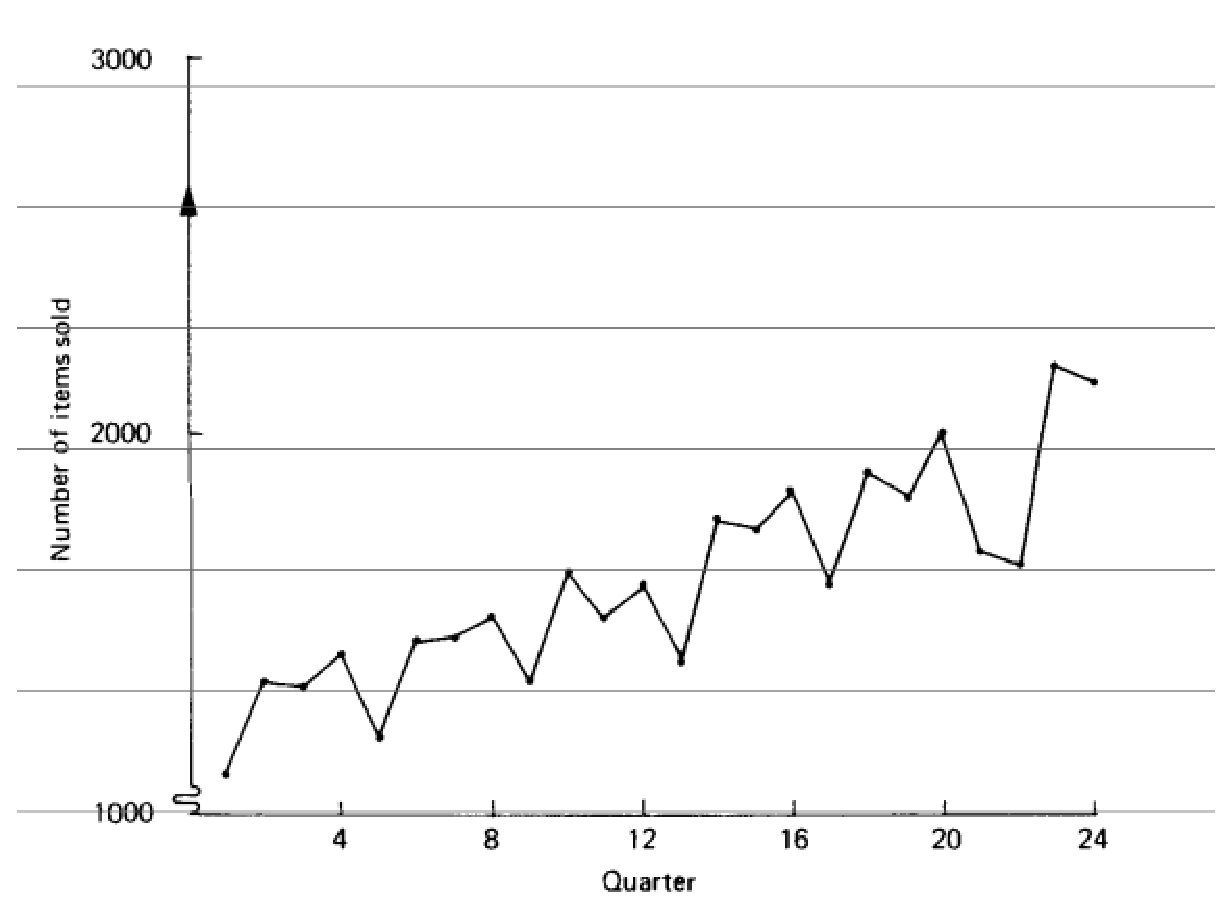
\includegraphics[scale = 0.50]{pictures/figure_5_2.eps}
\caption{Čtvrtletní prodeje vybrané společnosti pokrývající období šesti let}
\label{figure_5_2}
\end{figure}

\subsection{Příklad 2}

Obrázek (5.3) představuje časovou řadu nově instalovaných telefonních zařízení, kterou Tomasek (1972) analyzoval pomocí Box-Jenkinsovy metody. Tomasek vyvinul model
\begin{equation}
(1 - 0.84 B)(1 - B^{12})(X_t - 132) = (1 - 0.60B)(1 + 0.37 B^12)Z_t,
\end{equation}
který byl schopen vysvětlit 99.4\% celkového rozptylu pozorovaných dat. Na základě tohoto zjištění doporučil Tomasek použít tento model také pro účely predikce.

Zkoumaná časová řada vykazuje neobvykle pravidelnou sezónnost. Ve skutečnosti 97\% jejího rozptylu lze vysvětlit pomocí lineárního trendu a pravidelné sezónnosti. V případě, kdy je rozptyl časové řady dán trendem a sezónností, je efektivita ARIMA modelu dána především diferencí, která je na ni aplikována před samotnou kalibrací. Jinými slovy, pro takto pravidelná data bude prakticky libovolná metoda poskytovat ``vynikající'' výsledky.

\begin{figure}[htp]
\centering
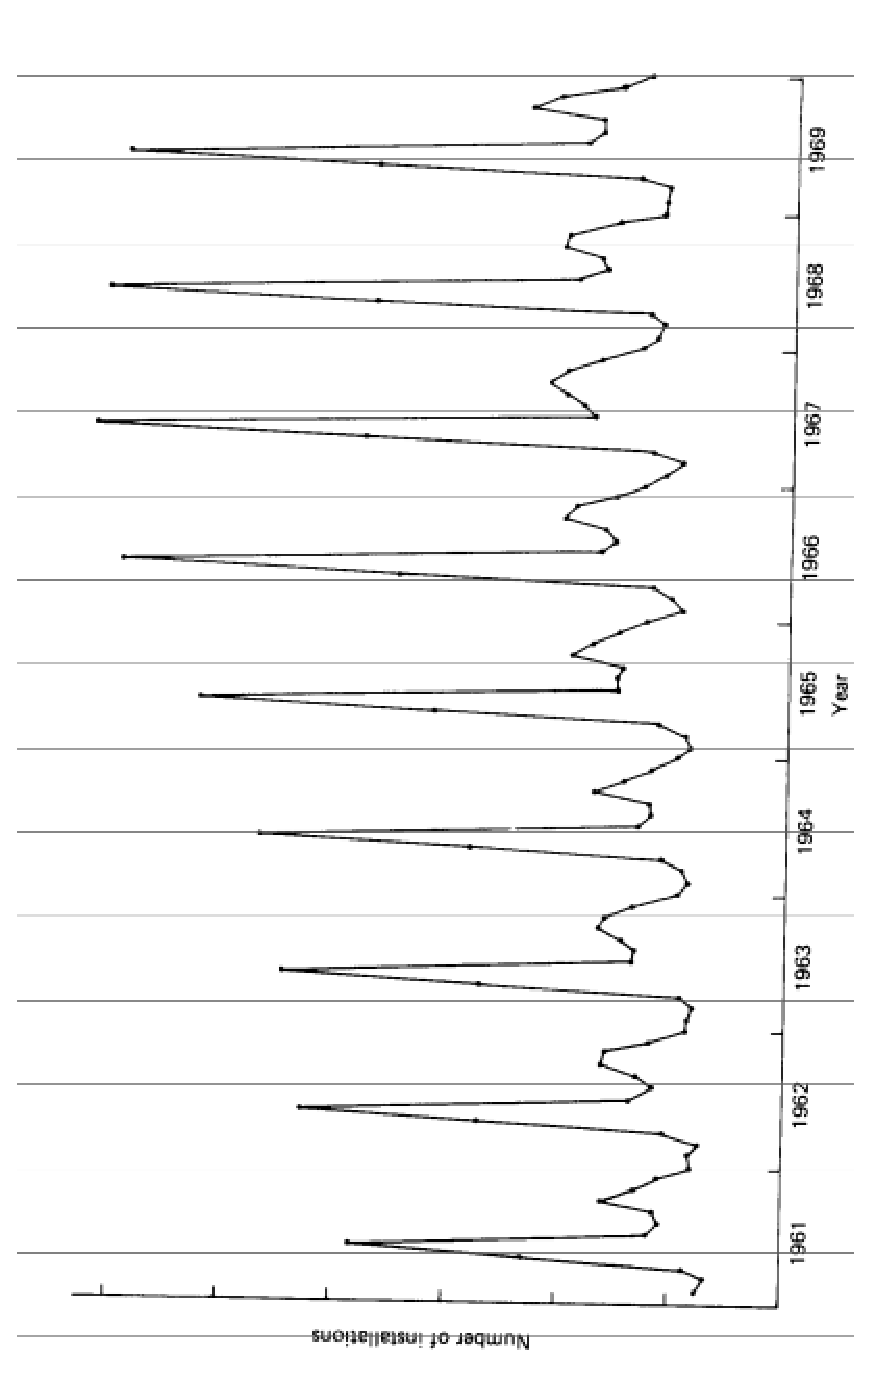
\includegraphics[scale = 0.50]{pictures/figure_5_3.eps}
\caption{Časová řada nově nainstalovaných telefonních zařízení}
\label{figure_5_3}
\end{figure}

\subsection{Příklad 3}

Obrázek (5.4) představuje čtvrtletní prodeje společnosti C pro 12 po sobě následujících let. Ačkoliv časová řada vykazuje známky sezónnosti, není tato sezónnost jinak pravidelná. D.L. Prothero analyzoval tuto časovou řadu pomocí Holt-Wintersovy a Box-Jenkinsovy metody. Ačkoliv byla Box-Jenkinsova metoda v porovnání s Holt-Wintersovou metodou o 3\% lepší při predikci na následující období\footnote{Měřeno formou směrodatné odchylky predikce oproti skutečně pozorovaným hodnotám.}, byla o 10\% horší při predikci na čtyři období dopředu.

Tento výsledek je typický pro Box-Jenkinsovu metodu, pro níž kvalita predikce klesá s prodlužujícím se časovým horizontem. Nicméně výsledek není typický v tom slova smyslu, že pro nepravidelnou časovou řadu, jako je ta na obrázku (5.4), dosahuje Box-Jenkinsova metoda horší predikce než konkurenční metody. Proto, má-li analytik dostatek času a zkušeností, může být aplikace Box-Jenkinsovy metody přínosná.

Tato časová řada také ilustruje možný přínos vícerozměrných prediktivních metod. Předpokládejme, že z původní časové řady na obrázku (5.4) odstraníme trend a sezónnost. Dále uvažujme časovou řadu zásob této společnosti, ze které taktéž odstraníme trend a sezónnost a navíc jsme ji zpozdíme o dvě čtvrtletí. Pokud pro predikci upravené časové řady čtvrtletních prodejů
použijeme lineární regresní model založený na upravené časové řadě zásob, bude takto získaná predikce vykazovat výrazně nižší směrodatnou odchylku než predikce založená na Holt-Wintersově či Box-Jenkinsově metodě.

\begin{figure}[htp]
\centering
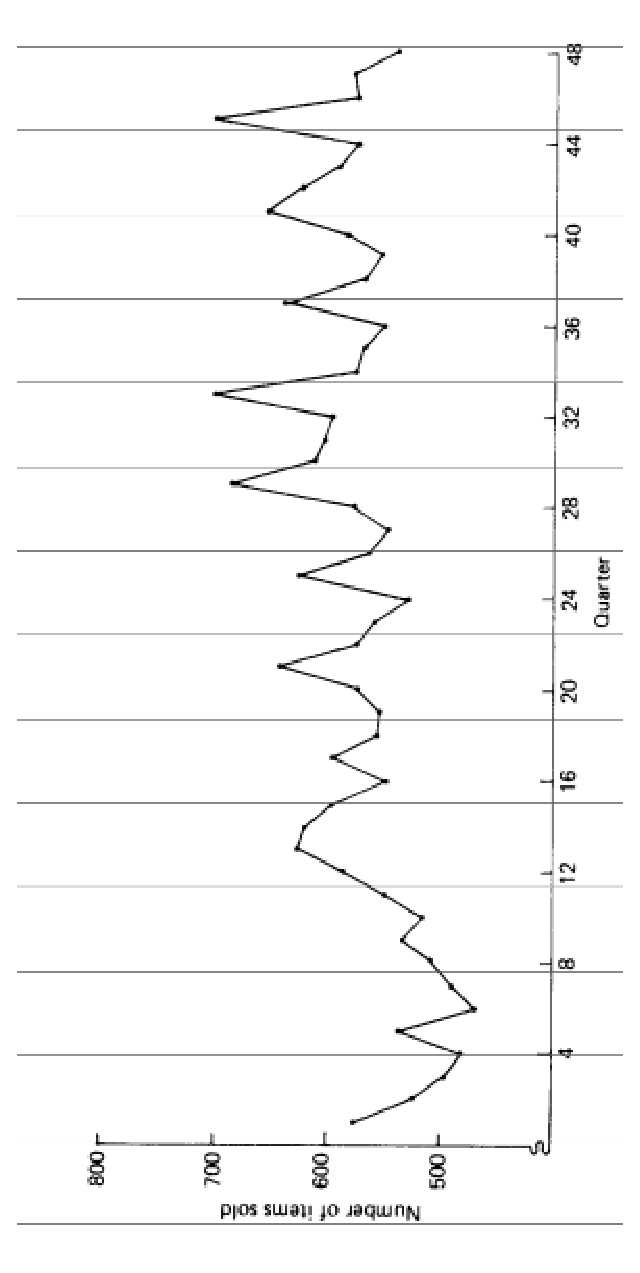
\includegraphics[scale = 0.50]{pictures/figure_5_4.eps}
\caption{Časová řada čtvrtletních prodejů společnosti C}
\label{figure_5_4}
\end{figure}

\section{Úvod do teorie predikce}

Kapitola 5 je specifickým výsekem z tzv. teorie predikce. Tato teorie má velký význam zejména pro oblast řízení, komunikace a výpočetních techniky. Následující text představuje pouze úvod do této problematiky.

V teorii predikce se vyskytují dva základní typy problémů. První typ problému spočívá v tom, že máme k dispozici časovou řadu $\{x_T, x_{T - 1}, ...\}$ a snažíme se odhadnout hodnotu $x_{T + m}$. Jedním ze způsobů, jak $x_{T + m}$ odhadnout, je použití funkce odhadu
\begin{equation}
\hat{x}_{T+m} = \sum_{j = 0}^{T - 1} c_j x_{T - j},
\end{equation}
která je lineární funkcí historických pozorování. Váhy $\{c_j\}$ jsou zvoleny tak, abychom minimalizovali střední hodnotu součtu čtverců reziduí $E(x_{T + m} - \hat{x}_{T + m})^2$. Wiener (1949) k problému odhadu vah $\{c_i\}$ přistoupil tak, že se snažil nalézt nejlepší funkci odhadu za předpokladu, že známe jak celou historickou řadu $\{x_t\}$ tak její autokorelační funkci. Box a Jenkins také použili lineární funkci odhadu, která byla optimální vzhledem ke zvolenému typu ARIMA procesu. Zatímco Wiener se praktickým postupem odhadu příliš nezabýval, Box a Jenkins (1979) poskytli návod, jak nalézt funkci odhadu, pokud je třeba odhadnout také autokorelační funkci.

Druhým typem problému je situace, kdy je signál $s(t)$ kontaminován šumem $n(t)$\footnote{V řadě případů je $n(t)$ důsledkem chyby měření.}, takže v praxi namísto $s(t)$ pozorujeme proces
\begin{equation}
y(t) = s(t) + n(t).
\end{equation}
Jak již asi tušíte, naším cílem je od sebe oddělit $s(t)$ a $n(t)$. Pokud máme k dispozici $y(t)$ až do času $T$, můžeme se pokusit o rekonstrukci signálu až do času $T$ popř. o predikci $s(T + \tau)$. Problematika rekonstrukce signálu se často nazývá vyhlazením popř. filtrací signálu. Často se předpokládá, že $s(t)$ a $n(t)$ jsou vzájemně nekorelované a že pro oba procesy známe jejich autokorelační funkce.


